%%%%%%%%%%%%%%%%%%%%%%%%%%%%%%%%%%%%%%%%%
% Journal Article
% LaTeX Template
% Version 1.4 (15/5/16)
%
% This template has been downloaded from:
% http://www.LaTeXTemplates.com
%
% Original author:
% Frits Wenneker (http://www.howtotex.com) with extensive modifications by
% Vel (vel@LaTeXTemplates.com)
%
% License:
% CC BY-NC-SA 3.0 (http://creativecommons.org/licenses/by-nc-sa/3.0/)
%
%%%%%%%%%%%%%%%%%%%%%%%%%%%%%%%%%%%%%%%%%

%----------------------------------------------------------------------------------------
%	PACKAGES AND OTHER DOCUMENT CONFIGURATIONS
%----------------------------------------------------------------------------------------

\documentclass[twoside,twocolumn]{article}

\usepackage{blindtext} % Package to generate dummy text throughout this template 

\usepackage[sc]{mathpazo} % Use the Palatino font
\usepackage[T1]{fontenc} % Use 8-bit encoding that has 256 glyphs
\linespread{1.05} % Line spacing - Palatino needs more space between lines
\usepackage{microtype} % Slightly tweak font spacing for aesthetics

\usepackage[german]{babel} % Language hyphenation and typographical rules

\usepackage[hmarginratio=1:1,top=32mm,columnsep=20pt]{geometry} % Document margins
\usepackage[hang, small,labelfont=bf,up,textfont=it,up]{caption} % Custom captions under/above floats in tables or figures
\usepackage{booktabs} % Horizontal rules in tables

\usepackage{lettrine} % The lettrine is the first enlarged letter at the beginning of the text

\usepackage{enumitem} % Customized lists
\setlist[itemize]{noitemsep} % Make itemize lists more compact

\usepackage{abstract} % Allows abstract customization
\renewcommand{\abstractnamefont}{\normalfont\bfseries} % Set the "Abstract" text to bold
\renewcommand{\abstracttextfont}{\normalfont\small\itshape} % Set the abstract itself to small italic text

\usepackage{titlesec} % Allows customization of titles
\renewcommand\thesection{\Roman{section}} % Roman numerals for the sections
\renewcommand\thesubsection{\roman{subsection}} % roman numerals for subsections
\titleformat{\section}[block]{\large\scshape\centering}{\thesection.}{1em}{} % Change the look of the section titles
\titleformat{\subsection}[block]{\large}{\thesubsection.}{1em}{} % Change the look of the section titles

\usepackage{fancyhdr} % Headers and footers
\pagestyle{fancy} % All pages have headers and footers
\fancyhead{} % Blank out the default header
\fancyfoot{} % Blank out the default footer
\fancyhead[C]{Running title $\bullet$ May 2016 $\bullet$ Vol. XXI, No. 1} % Custom header text
\fancyfoot[RO,LE]{\thepage} % Custom footer text

\usepackage{titling} % Customizing the title section

\usepackage{hyperref} % For hyperlinks in the PDF


\usepackage[utf8]{inputenc}
\usepackage{graphicx}

%----------------------------------------------------------------------------------------
%	TITLE SECTION
%----------------------------------------------------------------------------------------

\setlength{\droptitle}{-4\baselineskip} % Move the title up

\pretitle{\begin{center}\Huge\bfseries} % Article title formatting
\posttitle{\end{center}} % Article title closing formatting
\title{Data Lakes} % Article title
\author{%
\textsc{Raphael Drechsler}\\[1ex] % Your name
\normalsize HTWK Leipzig \\ 
\normalsize Fakultät Informatik, Mathematik und Naturwissenschaften\\ 
\normalsize Studiengang Informatik Master - Matrikelnr. 69872\\% Your email address
%\and % Uncomment if 2 authors are required, duplicate these 4 lines if more
%\textsc{Jane Smith}\thanks{Corresponding author} \\[1ex] % Second author's name
%\normalsize University of Utah \\ % Second author's institution
%\normalsize \href{mailto:jane@smith.com}{jane@smith.com} % Second author's email address
}
 \date{30.30.2018} % Leave empty to omit a date
\renewcommand{\maketitlehookd}{%
\begin{abstract}
\noindent 
Der Begriff des Data Lakes ist 2010 entstanden und wurde in den letzten Jahren stark ''gehyped''.\cite{src1} \cite{src2} \cite{src3} Es haben sich viele verschiedene Konzepte und Ansichten zum Thema entwickelt. Im Internet findet man bei einer Recherche zum Thema Data Lake von einem existierneden Unternehmen, welches sich ''the Data-Lake-Company'' nennt\cite{dlc}, bis hin zu einem Blogeintrag, der die Frage ''Are Data Lakes Fake-News?'' mit ja beantwortet\cite{src4} eine ganze Menge. Dabei wird die Frage danach, was ein Data Lake ist, von den verscheidenen Quellen nicht eindutig beantwortet. Auch gibt es zum Zeitpunkt des Erstellens dieses Dokumentes in der deutschsprachigen Wikipedia nock keinen Eintrag zu diesem Thema. Die Motivation dieses Abstracts besteht also darin, die bestehenden Unklarheiten zu beleuchten; zu klären was ein Data-Lake ist und sich mit der Frage ''Are Data Lakes Fake-News'' auseinanderzusetzen.
\end{abstract}
}

%----------------------------------------------------------------------------------------

\begin{document}

% Print the title
\maketitle

%----------------------------------------------------------------------------------------
%	ARTICLE CONTENTS
%----------------------------------------------------------------------------------------

\section{Definitionsfrage ''Data Lake''}
\lettrine[nindent=0em,lines=2]{D}er Begriff des Data Lakes wurde erstmalig von James Dixon (CTO von Pentaho \footnote{Pentaho gehört seit September 2017 dem Unternehmen Hitachi Vantara an}) geprägt. Auf seinem Blog \cite{src5}  und in mehren auf Youtube veröffentlichten Videos \cite{src6} stellt Dixon damals die von Pentaho angebotene Hadoop-basierte Big-Data-Lösung vor. Im Rahmen dieser Vorstellung stellt er auch das Prinzip vor, auf welchem die Solution basiert: Den Data Lake.\\
Dixon's Erläuterung des Prinzips beginnen damit, dass er durch Pentaho betrachtete Big-Data-Szenarien betrachtet und folgende gemeinsame Eigenschaften ableitet. 
\begin{itemize}
	\item Es liegt ein großes Datenvolumen vor, welches zu analysieren ist
	\item Die Daten entspringen einer Quelle
	\item Die Daten liegen in ihrer rohen Form vor (können also strukturiert, semi-strukturiert und un-strukturiert sein)
	\item ggf. sind die Daten angereichert (bspw. Anreichern von Weblogs um Geocodes)
\end{itemize}

\noindent Liegt ein Daten-Volumen vor, auf welches diese Eigenschaften zutreffen, handelt es sich Dixon nach um einen Data Lake. Im Weiteren nennt Dixon zusätzliche Eigenschaften eines solchen Data Lakes. Im Kern der Betrachtung steht dabei, dass der Data Lake als Datenvolumen verschiedenen Anwendern über verschiedene Unternehmensbereiche bekannte und unbekannte (wenn auch kleinere) Fragen beantworten kann und es daher sinnvoll ist, dieses Datenvolumen für spätere Analysen abzuspeichern.\\
Der von Dixon ausgeführte bildliche Vergleich macht diesen Umstand und die Vorstellung davon, was ein Data Lake ist, noch deutlicher.

\begin{figure}[h]
	\centering 
	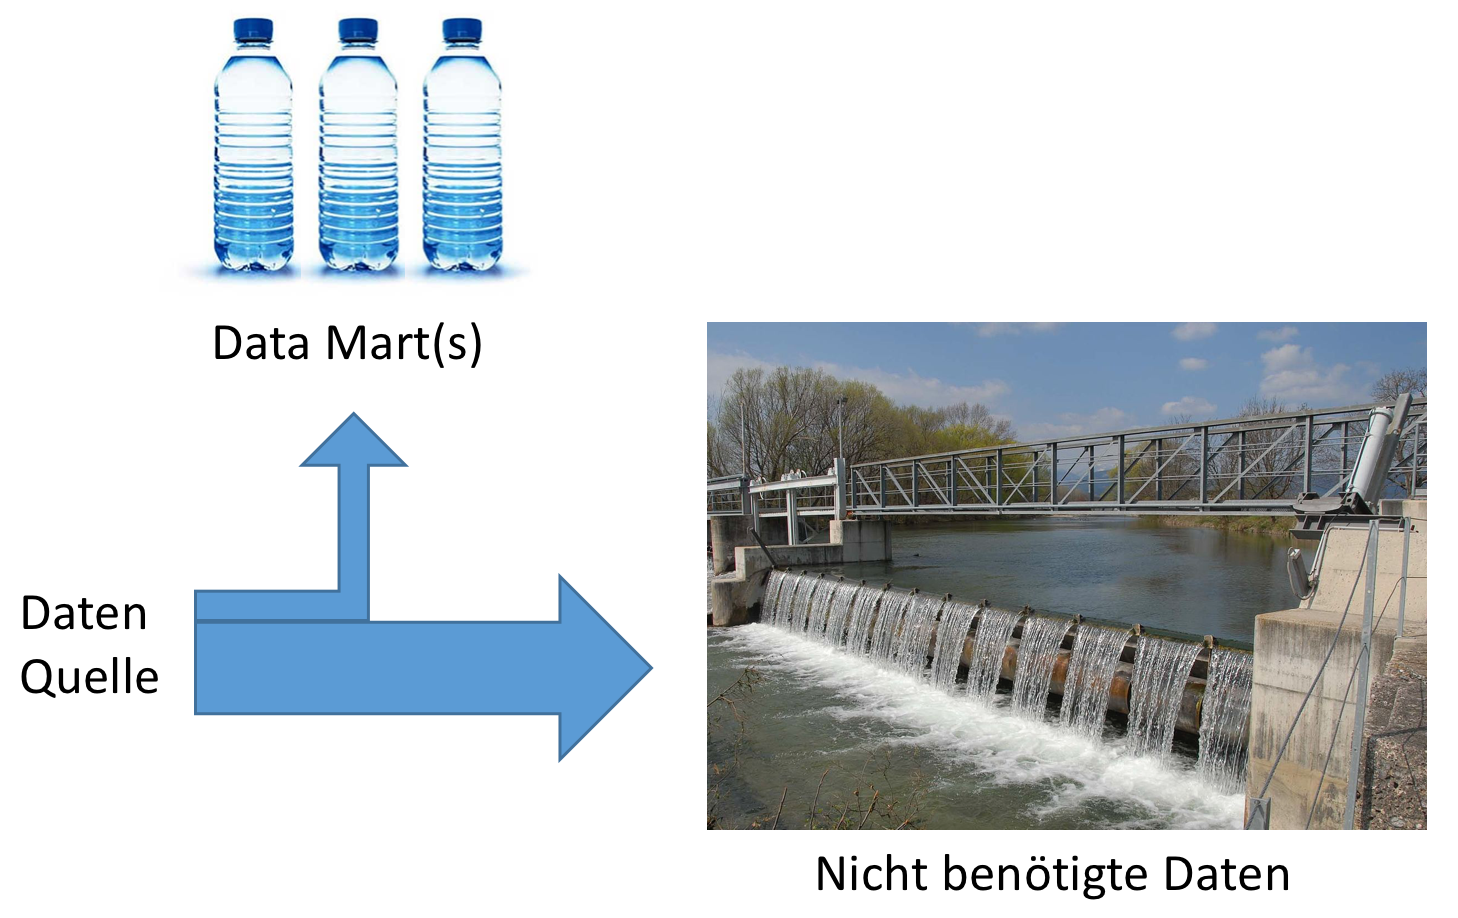
\includegraphics[width=0.4\textwidth]{img/p1} 
	\caption[DRT]{DRT \textit{nach} \cite{src6}}	
\end{figure}

Die Verbildlichung setzt bei den Data Marts an und stellt diese als fertig abgefüllte Mineralwasser-Flaschen dar. Das Wasser für diese Flaschen wurde aus einer Datenquelle gewonnen, bereinigt, aufbereitet und für den finalen Verwendungszweck abgepackt. Der Teil des Wassers (der Großteil), welcher nicht in die Data Marts eingegangen ist, fließt einfach ab. (Siehe Abb. 1)\\
Das Konzept des Data Lakes setzt an dieser Stelle an. Unter der Annahme, dass auch der Teil des Wassers, welcher abfließt, wertvolle Informationen enthalten kann, wird das Datenvolumen als Data Lake persistiert. Aus diesem lassen sich dann die Data Marts beliefern. Zusätzlich ist es dadurch möglich per Ad-Hoc-Query oder Report direkt auf das Datenvolumen zuzugreifen und somit zuvor unbekannte Fragen beantworten zu können. Zudem können Data Lakes wiederrum als Datenquellen für Data Warehouses genutzt werden. Es ergit sich das folgende Bild:

\begin{figure}[h]
	\centering 
	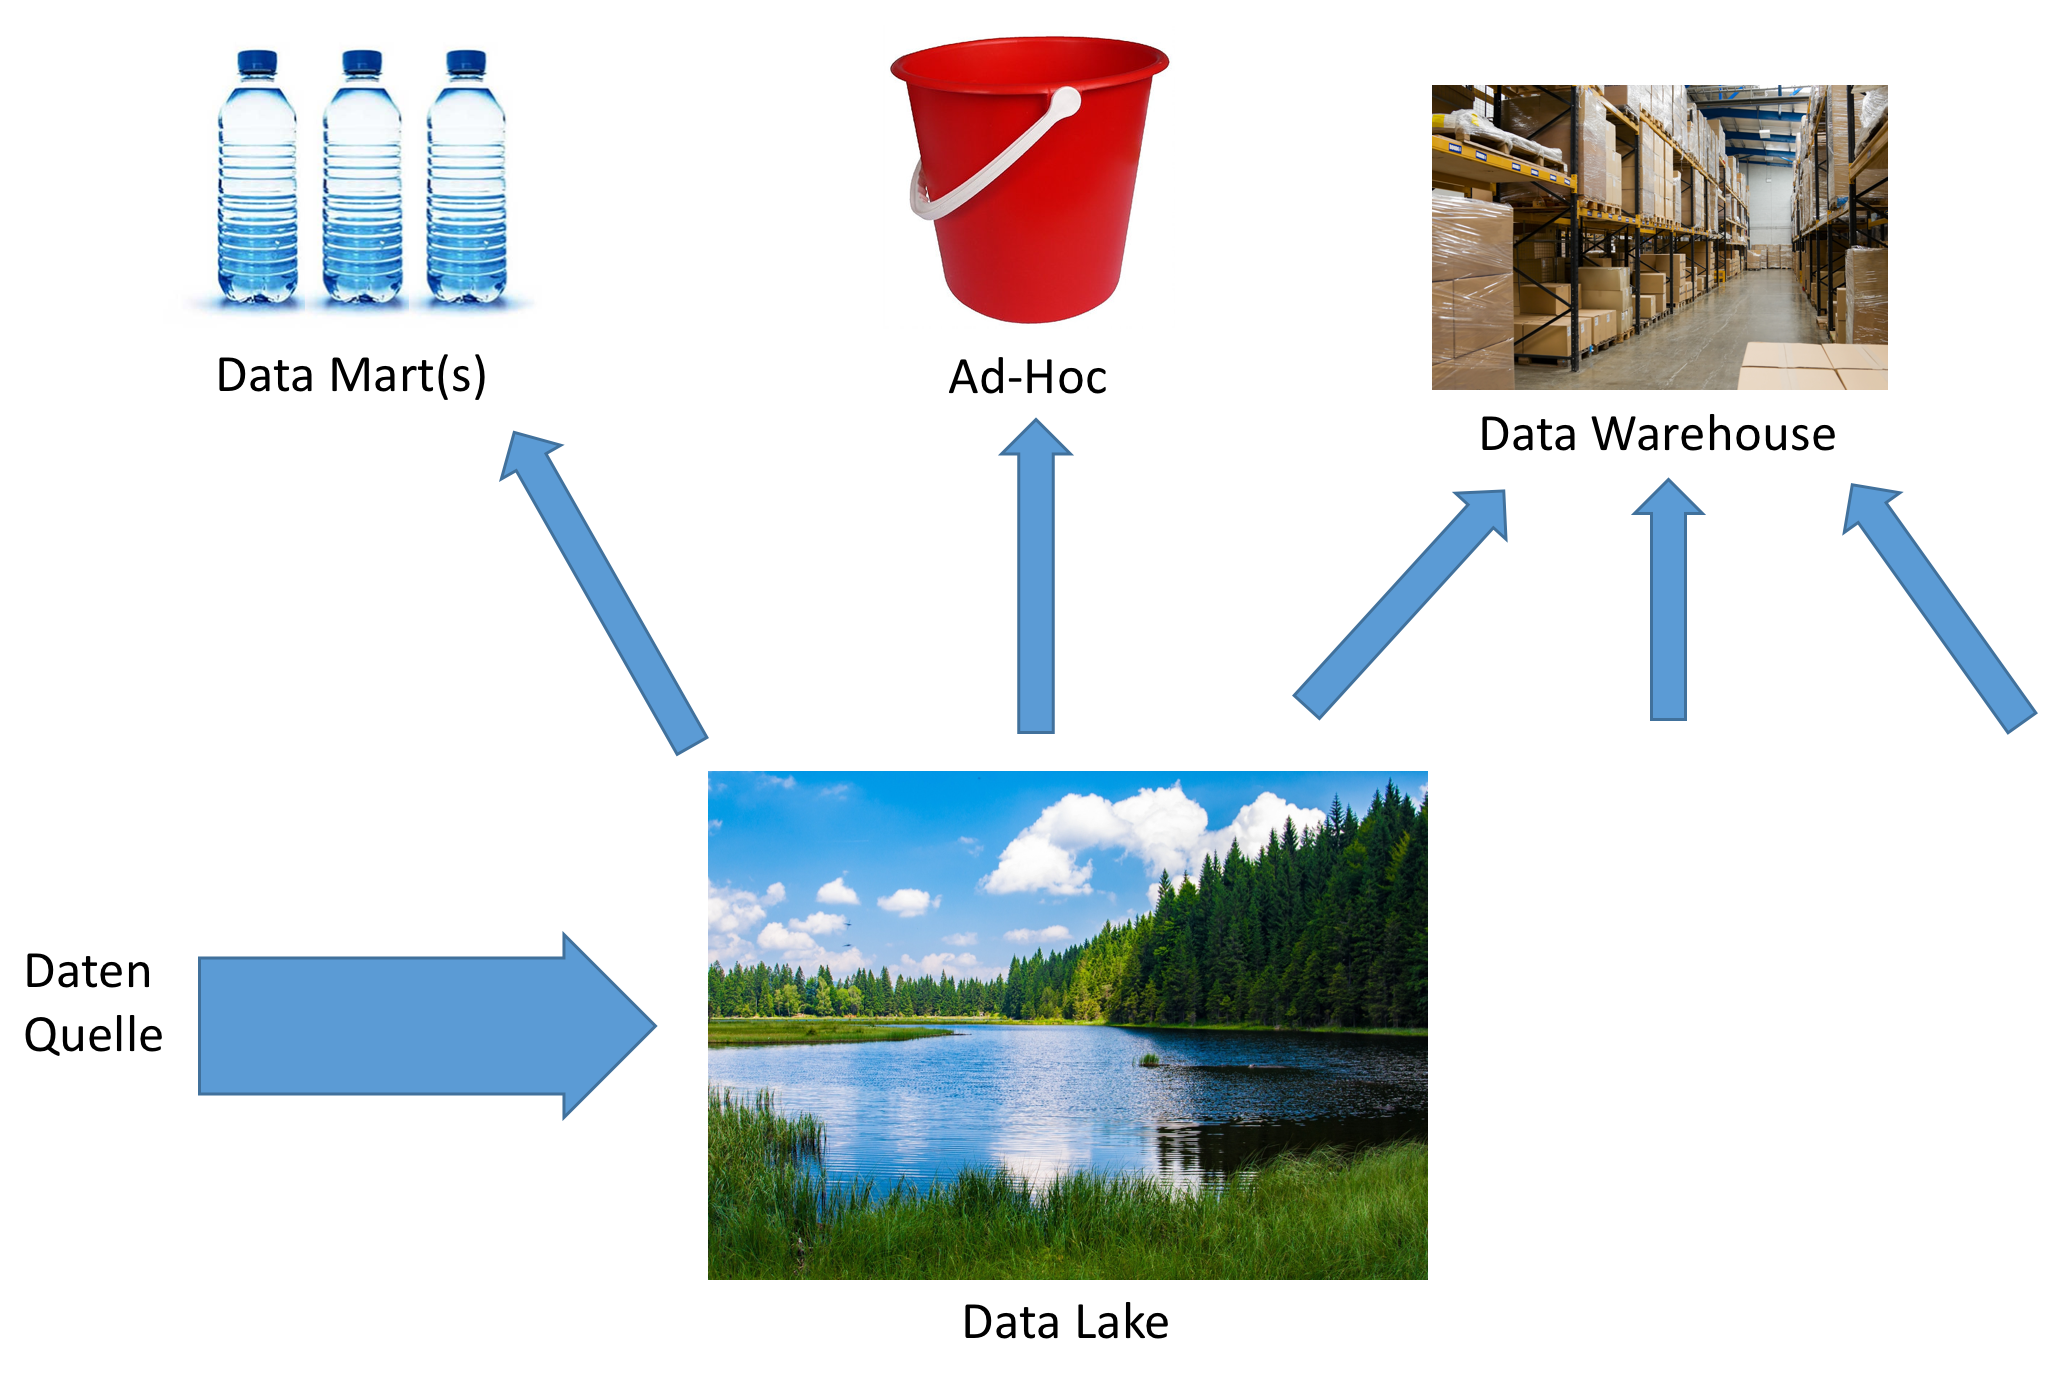
\includegraphics[width=0.4\textwidth]{img/p2} 
	\caption[DRT]{DRT \textit{nach} \cite{src6}}	
\end{figure}


Anmerkung zu extra-Pfeilen Data-Mart

Entsprechend folgt die Pentaho-Architektur 2010.

\begin{figure}[h]
	\centering 
	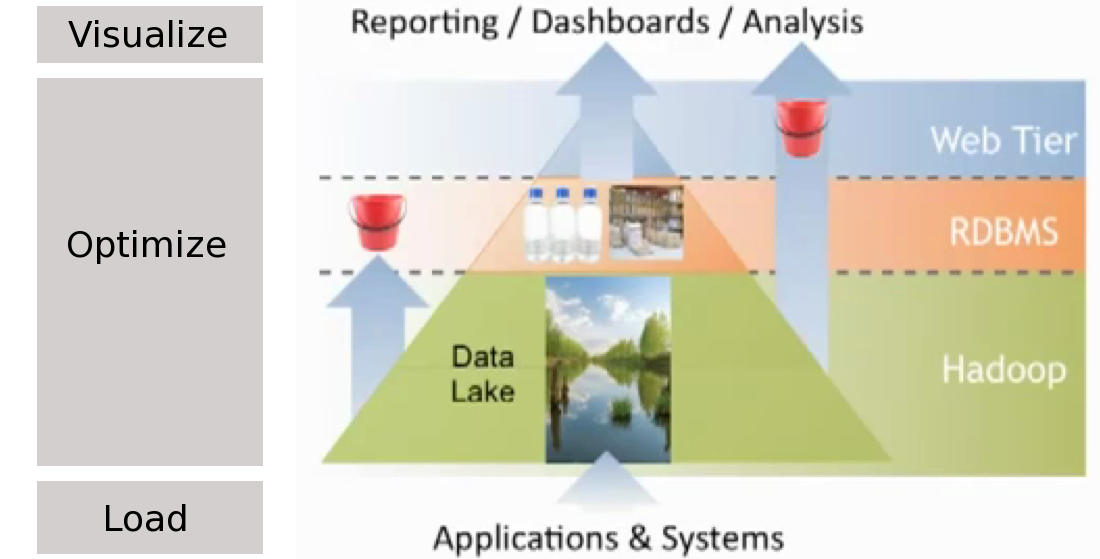
\includegraphics[width=0.4\textwidth]{img/p3} 
	\caption[DRT]{DRT \textit{nach} \cite{src6b}}	
\end{figure}

Die drei Schichten werden hier erstmalig gezeigt und sind klar.

Damit wars das an Definition. Niocht sehr genau. Weitere Unterkonzepte und Lösungen entstanden. Es gibt keinen einheitlichen Begriff.\cite{src7}

\section{Wie funktioniert ein Data Lake?}
Begriffe die sich gefestigt haben.

\paragraph{Aufbau und Workflow}
Aufbau
Analog zu Dixon Aufbau in drei Schichten.\cite{src8} \cite{src9}
\begin{itemize}
	\item F
	\item P u S
	\item Viz
\end{itemize}
Dabei wird P und S gelegentlich synonym als Data Lake bezeichnet, was von Dixon abweicht.

Workflow

Zusammengefasst wiefolgt:

\begin{figure}[h]
	\centering 
	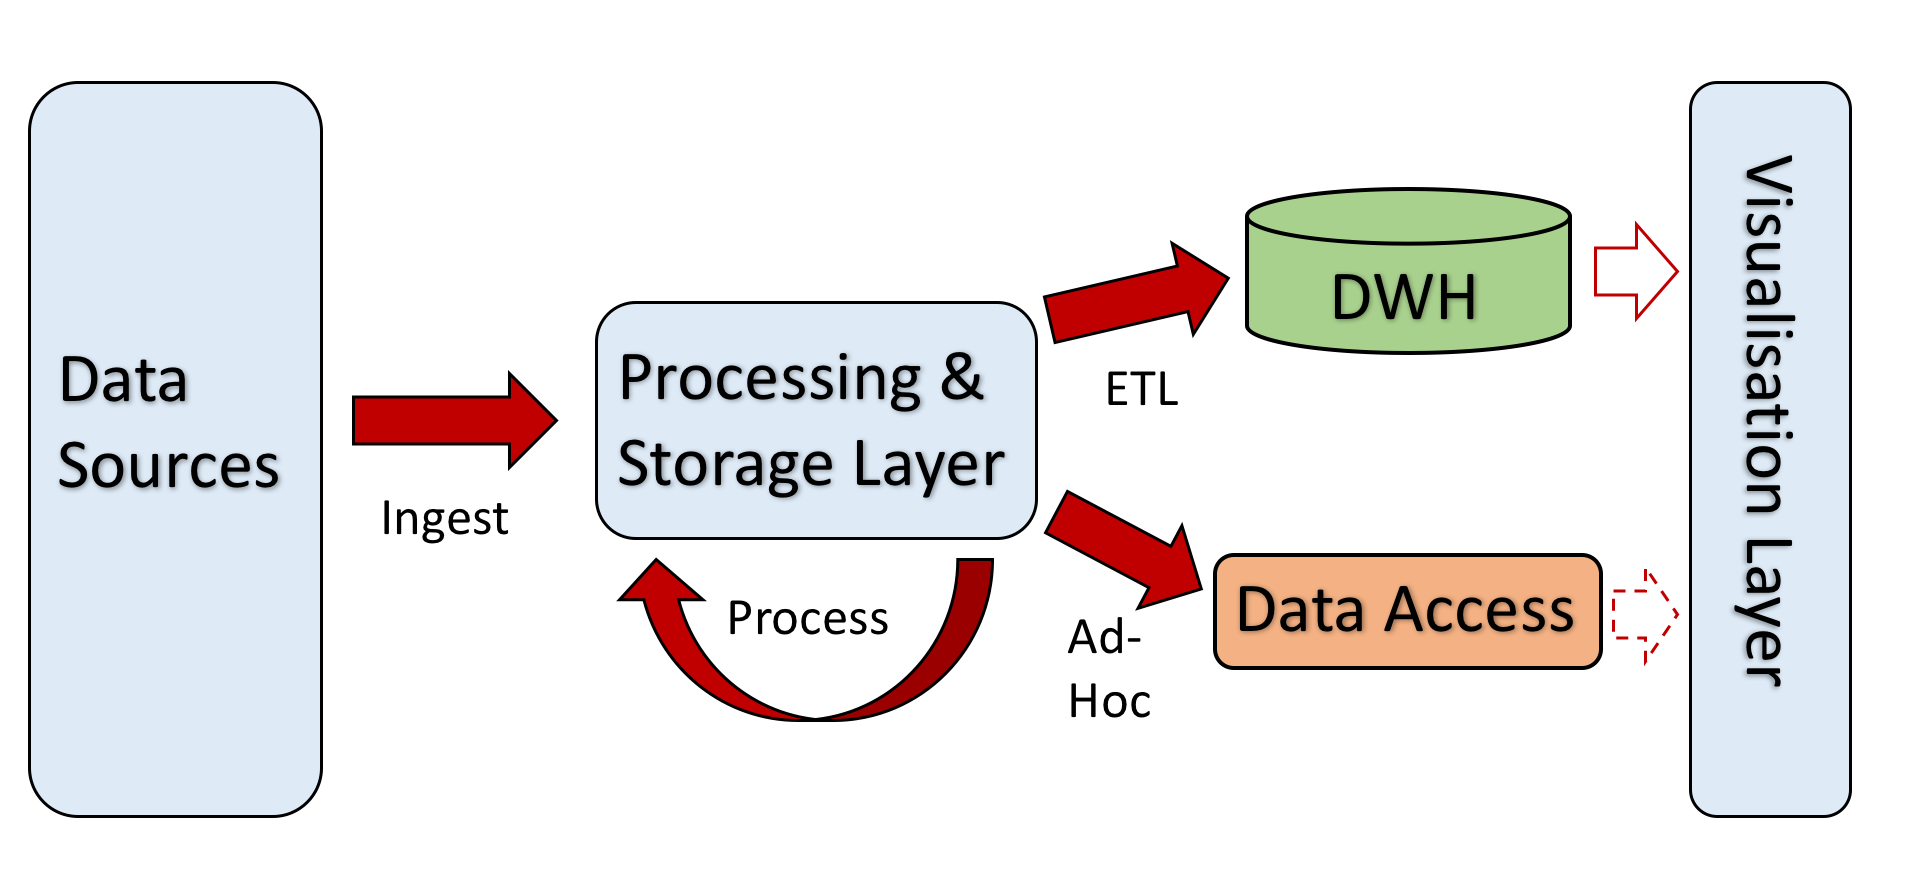
\includegraphics[width=0.4\textwidth]{img/p4} 
	\caption[DRT]{DRT \textit{nach} \cite{src9}}	
\end{figure}


Brauchen Daten nach DL\\
Brauchen aufbereiten des Wassers. Hierbei spielt die Rolle des Data Scientist eine Rolle.\cite{src8}\\
Dann zur Verfügung stellen\\
Oben: Visaulisierung. Was dabei visualisiert wird variiert von Sol zu Sol.


\paragraph{Storage}
QUELLEN : 8, ?
\paragraph{Ingestion}
QUELLEN : 8, 10, 11
\paragraph{Process}
QUELLEN : 8, 12
\paragraph{Consumption}
QUELLEN : 8, 12
\paragraph{Monitoring}
QUELLEN : 8, ?
\paragraph{Data Governance}
QUELLEN : 8, 12


\section{Data Swamps: Kritik am Data Lake}
Mögliche Darstellungen die es so gibt:
\begin{itemize}
	\item Sumpf: findest nix und gehst unter \cite{src3}
	\item Finnland: heterogen, nicht zu inregreiren \cite{src13}
	\item Flohmarkt: Findest alles aber wie sucht man?, wem kann man vertrauen? Qualität? \cite{src12}
\end{itemize}

Gartners wesentliche Punkte\\
Aufstieg Data Lake durch scheinbar Löung im Problem. Konzept hat aber Lücken und wenig Substanz. Es kommt zu undergoverned und Meta-Daten-losen Hadoop-Clustern. Dies ist im wesentlichen das was unter dem Begriff Data Swamp verstanden wird.\cite{src3}

Battle: Gartner vs. Dixon und \\
Dixon setzt sich zur Wehr. Insbesondere Anzahl Quellen: Wassergartenarchitektur.\cite{src15} Auch Metadaten. Macht dazu keine Angaben, aber sagt, dass es nicht heißt, dass nicht.\cite{src14} Auf jeden Fall festhalten: ungenaue Definition.\

Neben diesem Problem ansehen, was in der Praxis passiert: Hier ist Sean Martin zu zitieren.\\
Es kommt generell zu dem Trend des Vorsichtiger werdens und die Flut kommen sehen. Paradigmenwechsel.\cite{src1}

\section{Fake-News! Existieren Data Lakes überhaupt?}
Blogeintrag nur nennen und erste Zeile zitieren.\cite{src4}\\

Nach Recherche lassen sich da schon ein paar Firmen finden, die Data Lake Lösungen anbieten.
Unter anderem zu nennen sind : Firma\cite{c1}, Firma\cite{c2}, Firma\cite{c3},...

Nach weiterer Recherche auch success-stories auffindbar. 
Zu nennen sind hierbei die Storys von Firma\cite{ss1}, Firma\cite{ss2}, Firma\cite{ss3}. Auch Zaloni hat Testemonial \cite{ss4}.

Im Bsp von UCI Health ist Lösung gut, weil \cite{src1}\cite{ss2} 

Also irgendwie schon.


Die wesentliche Frage ist allerdings die Definitionsfrage.\\
Selber Schluss im Blogeintrag. Lösung die dem Paradigma grundlegend folgen gibt es. Jetzt im Auge des Betrachters ob man das Kind beim Namen nennt oder nicht.


%------------------------------------------------


%------------------------------------------------



%----------------------------------------------------------------------------------------
%	REFERENCE LIST
%----------------------------------------------------------------------------------------

\bibliographystyle{unsrt}
\bibliography{bib.bib} % The file containing the bibliography

%----------------------------------------------------------------------------------------

\end{document}
